\chapter{浮動小数点数と区間演算} \label{chap:interval}


%
%----------------------------------------------------------------------------------------------------------------------------------------------
%----------------------------------------------------------------------------------------------------------------------------------------------
%----------------------------------------------------------------------------------------------------------------------------------------------
\section{\texorpdfstring{$5$}{5}次の代数方程式の解の品質保証を手計算でやってみよう}\label{sec:5nonlinear}
まず，数値計算を用いた方程式の品質保証法の感覚をつかんでもらうために，$5$次の代数方程式
\begin{align}
	\label{eq:five_order_equation}
	\mbox{Find} ~ x \in {\mathbb R} ~ \mbox{s.t.} ~ -5 x^5 + 5 x^4 + 5 x^3 + 6 x^2 + 6x + 5  = 0
\end{align}
の解を考えてみましょう．
ここで，${\mathbb R}$は実数全体の集合を意味し，s.t.はsuch thatの略語です．
すなわち，「方程式\eqref{eq:five_order_equation}を満たす解を実数全体から探せ」という問題です．
$5$次の代数方程式の解は因数分解によって解ける場合もあるし，そもそも実数に解がない場合もあります．
そして，数値計算を用いて方程式\eqref{eq:five_order_equation}の近似解を求める手法は多く知られています．
「答えがすぐにわからない」，「そもそも答えが存在するかもわからない」，「数値計算法で近似的に求められる」ので，はじめて品質保証を行うには持ってこいです．

先に答えを見せてしまうと，この方程式\eqref{eq:five_order_equation}に対して私の手元のコンピュータで実際に品質保証まで含めて解いてみると結果は区間
\begin{align*}
[ 2.006595606321886, 2.006595606321888]
\end{align*}
内に真の解が必ず一意に存在することを保証できました．
すなわち，真の解の上位15桁は「$2.00659560632188$」であることがわかります．
この結果はコンピュータを使って計算しましたが，本章では流れをつかんでもらうために手計算で計算していきたいと思います．


では，方程式\eqref{eq:five_order_equation}に対して，手計算で数値計算の品質保証の流れをつかんでみましょう．
まず，今回の例で使う重要な定理を紹介します．
定理を紹介したのちに，一歩ずつ定理の使い方を解説しますので，定理だけで理解する必要はありません．

\begin{Thm}\label{thm:Basic_Theorem_five_order_nonlinear}
	$\hat{x} \in {\mathbb R}$を与えられているとする($\hat{x}$はコンピュータで求めた近似解をイメージしており，なんでも構いません!)．
	$f:{\mathbb R} \rightarrow {\mathbb R}$を与えられた関数とする．(問題となる方程式を$f(x) = 0$と書き直したときの関数$f$です!)．	
	関数$f$は$\hat{x}$で微分可能とし$f'[\hat{x}]$と表記する．
	$f'[\hat{x}]$は逆を持つと仮定する．
	$\eta$を
	\begin{align*}
		| f'[\hat{x}]^{-1}f(\hat{x}) | \le \eta
	\end{align*}
	を満たす定数とする．
	また，関数$f$は$\hat{x} + v, ~ \forall v \in [-2 \eta, 2 \eta]$で微分可能とする．
	
	定数$K$を不等式
	\begin{align*}
	|  f'[\hat{x}]^{-1} \left( f'[\hat{x}] -  f'[\hat{x} + v] \right) | \le K, ~ v \in [-2 \eta, 2 \eta]
	\end{align*}
	を満たす定数とする．
	もし$2K\le 1$ならば，$f(x) = 0$を満たす解を$x^*$とすると
	\begin{align*}
		| x^* - \hat{x} | \le \frac{ \eta }{1 - K} =: \rho
	\end{align*}
	となり，$[ \hat{x} - \rho, \hat{x} + \rho ]$内に$x^*$は存在する．
	そのうえ，$[ \hat{x} - 2 \eta, \hat{x} + 2 \eta ]$内で一意である．
\end{Thm}


第\ref{chap:basic_theorem}章の目標が，この定理\ref{thm:Basic_Theorem_five_order_nonlinear}をものすごく一般化した定理\ref{thm:Basic_Theorem}の証明ですので，ここでは証明をつけずに利用だけしたいと思います．
数値計算の品質保証では上のような定理\ref{thm:Basic_Theorem_five_order_nonlinear}の十分条件を満たすか確認をしていきます．
これから一つずつ設定/計算/十分条件の確認を行っていきますので，定理\ref{thm:Basic_Theorem_five_order_nonlinear}のどこにあたる部分か，迷わないように定理を見比べながら読み進めてください．

まず，品質を保証したい近似解$\hat{x}$を決めます．
今回は手計算で話を進めるために，
\begin{align*}
	\mbox{近似解} ~ \hat{x} = 2
\end{align*}
とします．
どんな近似解が来ても品質保証を行い判断をしなければならないために，最初の近似解はなんでも良いです．
もちろん，この近似解が良ければ品質が良いものと判断されます．


次に，方程式\eqref{eq:five_order_equation}を$f(x) = 0$の形に書き直します．
すなわち，
\begin{align*}
	f(x) = -5 x^5 + 5 x^4 + 5 x^3 + 6 x^2 + 6x + 5
\end{align*}
とすれば良いですね．
また，$f$の微分も必要になります．
$f$の$y$における微分は
\begin{align*}
	f'[y] = -25 y^4 + 20 y^3 + 15 y^2 + 12 y + 6
\end{align*}
となります．
もちろん$y \in {\mathbb R}$と取れるので，$f$は実数全体で微分可能です．


続いて，定数$\eta$を計算する準備として，近似解$\hat{x}$における残差$f(\hat{x})$と微分値$f'[\hat{x}]$を計算します:\\
残差$f(\hat{x})$:
\begin{align*}
	f( \hat{x} ) = -5 \times 2^5 + 5\times 2^4 + 5\times 2^3 + 6 \times 2^2 + 6\times 2 + 5 = 1
\end{align*}
近似解$\hat{x}$における$f$の微分値$f'[\hat{x}]$
\begin{align*}
	f'[\hat{x}] = -25 \times 2^4 + 20 \times 2^3 + 15 \times 2^2 + 12 \times 2 + 6 = -150
\end{align*}

次に，近似解$\hat{x}$における$f$の微分値が逆を持つことを確認します．
今回は$f'[\hat{x}] \neq 0$であるため$f'[\hat{x}]$は逆を持ちます．

次にNewton法の修正量$f'[\hat{x}]^{-1} f(\hat{x})$の絶対値を計算し，$\eta$を計算します．
\begin{align*}
	| f'[\hat{x}]^{-1} f(\hat{x}) | = \frac{1}{150} =: \eta
\end{align*}

次に，定数$K$の計算です．
関数$g$を
\begin{align*}
	g(y) =& 1 - \left(-\frac{1}{150}\right) \left( -25 y^4 + 20 y^3 + 15 y^2 + 12 y + 6 \right), ~ \forall y \in \left[2-\frac{1}{75}, 2 + \frac{1}{75} \right] \\
	=& -\frac{1}{150} \left( y - 2 \right) \left(25 y^3 + 30 y^2 + 45 y + 78 \right), ~ \forall y \in \left[2-\frac{1}{75}, 2 + \frac{1}{75} \right]
\end{align*}
とすると，定数$K$は
\begin{align*}
	|  g(y) | \le K, ~ y \in [\hat{x}-2 \eta, \hat{x} +2 \eta]
\end{align*}
となるため，関数$g$の定義域を$[\hat{x}-2 \eta, \hat{x} +2 \eta]$としたときの最大値と最小値を求めれば良いです．
一応，関数の最大値と最小値の求め方は高校生の学習範囲ですが，値が綺麗ではないので最大値と最小値を求めるのは大変です．
そのため結果だけ書くと
\begin{align*}
	-\frac{4170083}{94921875} \le g(y) \le \frac{4065457}{94921875}, ~ \forall y \in [\hat{x} -2 \eta, \hat{x} + 2 \eta]
\end{align*}	
となります．
よって，定数$K$は
\begin{align*}
	K = \frac{4170083}{94921875}
\end{align*}	
とすれば良いです．


定数$K$が求まったら十分条件
\begin{align*}
	2 K \le 1
\end{align*}
の確認です．
もし，ここで1以下でなかった場合は品質保証が失敗になり，そもそも近似解の近くに解が存在するかどうかわかりません．
今回の問題では，
\begin{align*}
	2 K = \frac{8340166}{94921875} \le 1
\end{align*}
となるので，近似解の近くに解が存在することが証明できます．
これで定理\ref{thm:Basic_Theorem_five_order_nonlinear}の十分条件はクリアです!
そのうえで，真の解を$x^*$と書くと，真の解と近似解の誤差は
\begin{align*}
	| x^* - \hat{x}  | \le \frac{\eta}{ 1 - K }
\end{align*}
となります．
今回の場合は
\begin{align*}
	| x^* - \hat{x}  | \le \frac{ \frac{1}{150} }{ 1 - \frac{4170083}{94921875} } = \frac{1265625}{181503584} \le 0.007
\end{align*}
となります．
また，区間
\begin{align*}
	[ 1.993, 2.007 ]
\end{align*}
内に真の解が存在していることも証明されました．
これで，定理\ref{thm:Basic_Theorem_five_order_nonlinear}の使い方の説明はおしまいです．
定理を使っている最中に，真の解がわかっている必要がなく，そのうえ，最後まで行っても真の解はわかりません．
しかし，最初に設定した近似解$\hat{x}=2$の近く(具体的には絶対誤差$| x^* - \hat{x}  | \le 0.007$)に解が存在することがわかりました．

ついでに，この誤差が大きいか，小さいかわかりやすいように誤差率もどきの上界も計算してみましょう．
誤差率の定義は
\begin{align*}
	\mbox{誤差率} = \left| \frac{  \mbox{真値} - \mbox{近似値}  }{ \mbox{真値} } \right| \times 100 [\%]
\end{align*}
です．
しかし，真の解$x^*$がわかっていないので分子の真値はわかりません．
そこで，数値計算の品質保証では，近似値の近くに真値があることから誤差率もどき
\begin{align*}
	\mbox{誤差率もどき} = \left| \frac{  \mbox{真値} - \mbox{近似値}  }{ \mbox{近似値} } \right| \times 100 [\%]
\end{align*}
をつかいます．
先ほどの例では誤差率もどき上界は
\begin{align*}
	\mbox{誤差率もどき} = \left| \frac{ x^* - \hat{x}  }{ \hat{x} } \right| \times 100 [\%] \le \frac{0.007}{2}\times 100 = 0.35 [\%]
\end{align*}
となります．
誤差率もどきの上界$0.35$\%が大きいか小さいかは，用途によって変わります．
もちろん要求する精度がもっと必要な場合は近似解を$2$としてはダメであり，もっと高品質な近似解を設定しなければなりません．

本節では定理\ref{thm:Basic_Theorem_five_order_nonlinear}の
\begin{itemize}
	\item $f'[\hat{x}]$が逆を持つこと
	\item 定数$\eta$の計算
	\item 定数$K$の計算
	\item 十分条件$2K \le 1$のチェック
	\item 絶対誤差の上界$\rho$
\end{itemize}
は手計算し，確認していきました．
ポイントは，近似解にどんな誤差が入っていようが関係なく，与えられた何でもいい近似解に対して検証できる点です．
しかし，もっと複雑な問題や大規模な問題に対応するためには，手計算では限界があるためにコンピュータの利用は必須になります．
そのために，定数$\eta$や$K$をコンピュータで正確に求めなければなりません．
そこで，本章では残りの節ではコンピュータを用いてある定数$\eta$や$K$を正確に求める方法として，ある種の集合演算である「浮動小数点数における区間演算」を導入します．
区間演算によって，浮動小数点数を扱う際に発生する誤差を考慮しながら計算することが可能になります．
それでは，浮動小数点数の正確な定義からはじめましょう．


%
%
%----------------------------------------------------------------------------------------------------------------------------------------------
%----------------------------------------------------------------------------------------------------------------------------------------------
%----------------------------------------------------------------------------------------------------------------------------------------------
\section{コンピュータで扱う小数: 浮動小数点数とは?}
コンピュータ上の計算と聞くと万能そうに聞こえますが，多くの場合，取り扱う数値を近似してしまいます．
例えば，円周率$\pi$をコンピュータで扱うにはどうすればよいか?と考えてみます．
まず，記号として$\pi$のように保持することができます．
しかし，$\pi$を記号としてそのまま処理できる演算はCPU上には実装されていないため，数値計算とは別分野の数式処理としてソフトウェア的にしか計算できません(数式処理ソフトの例としてMathematicaなどがあります．)．
それでは，$\pi$を小数で保持しようとしても，$3.141592...$と無限の桁が続くため，コンピュータのメモリーも無限に必要になります．
$\pi$を使って演算したいのに，$\pi$をそのまま保持することはできないので，現状では，「有限桁に打ち切った小数」としてコンピュータで扱います．
さらには，コンピュータは内部では$0$と$1$の2進数で表される決められた一定の長さのビット列でデータを保持します．
そのため，「決められた一定の長さのビット列で表現する有限桁に打ち切った小数」の取り扱い方に関する議論が必要です．
色々な規則が開発されているが，今，現在，多くのPCに実装されているCPUはIEEE 754 標準という規格に基づいています．
IEEE 754 標準では，浮動小数点数に関する技術規格が制定されています．
IEEE 754 標準の詳細を述べる前に，品質を扱うからこそ知っておいてほしい重要なことがあります．
上の例で扱った$\pi$は「無理数なんだから，コンピュータで実際に持てなくても仕方ない」って思っている読者に是非聞いてほしいことです．
例えば，IEEE 754標準では十進数で$1.1$は厳密には表現できません．
すなわち，何かしらのプログラミング言語で，浮動小数点数として1.1を保持しようとすると，1.1を近似して保持をします．
そのために，計算する以前にすでに誤差が発生してしまいます．


IEEE 754 標準には，singleとdoubleというフォーマットがあります．
singleは32 bitの長さで近似して保持し，doubleは64 bitの長さで近似して保持します．
詳細は以下の規格書をみてください:

\begin{center}
{\small\url{http://ieeexplore.ieee.org/stamp/stamp.jsp?tp=&arnumber=4610935}}
\end{center}

本章では，IEEE 754 規格の簡単な紹介と，品質保証に必要となる丸め変更について説明します．
前述したとおりIEEE 754 規格では\textit{single}と\textit{double}という$2$進数の浮動小数点数のフォーマット
\[
	(-1)^s \times 2^e \times m
\]
が規格化されています．
ここで，$s, e, m$はそれぞれ

\begin{enumerate}[label=\alph*), leftmargin=15mm, topsep=2pt, itemsep=0pt, parsep=0pt]
\item 符号ビット $s$ : $1$ bit ($0$ あるいは $1$)
\item 指数部$e$ : $e_{\min} \le e \le e_{\max}$となる整数
\item 仮数部$m$ : 正規化された形式 $d_0.d_1 d_2 \cdots d_{p-1}$で表現される．ただし，$d_i$は$0$ or $1$.
\end{enumerate}
\noindent です．
$e_{\max}, e_{\min}, p$は\textit{single}と\textit{double}で変化し，表\ref{3:table_val}のように定められています(ただし，$e_{\min} := 1 - e_{\max}$です)．

\begin{table}[htb]
\centering
\caption{指数部と仮数部}\label{3:table_val}
\begin{tabular}{|c | c c |}
\hline
Parameter & single & double \\ \hline
$p$          & 24 bit    &    53 bit   \\ \hline
$e_{\max}$     & 127   &    1023 \\   \hline
\end{tabular}
\end{table} 

また，図\ref{3:fig_float}に\textit{Single}の場合の表現を図示します．
ポイントは，正規化数と呼ばれる状態では常に$d_0 = 1$としておき，$d_1$から記憶させています．
これにより$1$ bit分だけお得に記憶できるため，「ケチビット」と呼ばれます．

\begin{figure}[htb]
 \begin{center}
  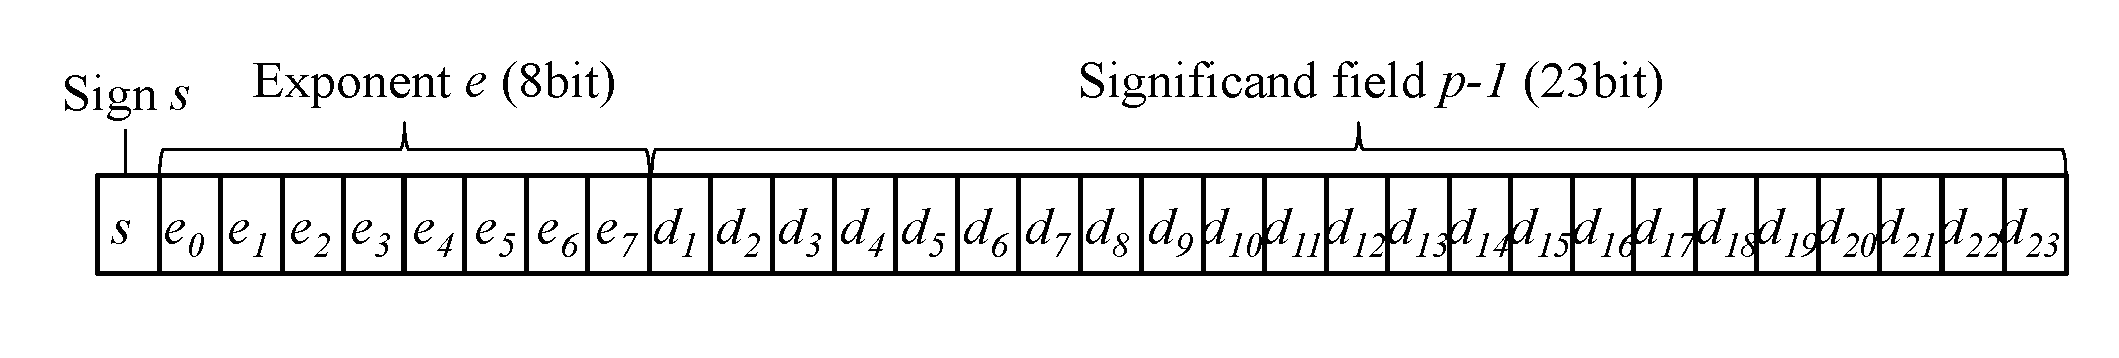
\includegraphics[width=\linewidth]{figs/3_fig_float.eps}
 \end{center}
  \caption{\textit{Single}の場合の表現方法}
 \label{3:fig_float}
\end{figure}

\Mondai
	10進数$7.25$を浮動小数点数に変換せよ．
	ただし，$p$は($d_0$も含め)$6$ bitとし，$e$は$3$ bitとする．\\

\Kaitou
	\begin{align*}
	7.25 &= (111.01)_2 \\
	&= (-1)^0 \times 2^2 \times (1.1101)_2
	\end{align*}
	ここで，$(\cdot)_2$は2進数を意味する．
	そのため，解答は
	\begin{align*}
	0 ~~ 010 ~~ 11010
	\end{align*}
	となる．\\

仮数部$p = 3$ bitとすると，上記の例題にある仮数部のビット$11010$は表現できないことに気が付くと思います．

${\mathbb{F}}$をIEEE 754 規格で定義された浮動小数点数の集合とします．
もちろん，${\mathbb{F}} \subset {\mathbb{R}}$であることに注意してください．
そのとき，IEEE 754 標準における切り捨てや切り上げなどの丸めは，$+ , ~ -, ~ *, ~  /, ~ \sqrt{\cdot} $ の\uwave{5つの演算結果に限り，丸めが定義}されています．
ここで注意点として，入力や出力，初等関数$\sin$などの丸めに関しては定義されていないので注意してください．
実際に，$\circ \in \{ +, -, \times, /  \}$としたとき，以下の例えば3つの丸めモードがあります(ちなみに，2008年に制定されたIEEE 754 規格では全部で5つの丸めモードがあります．):

\begin{enumerate}[label=\alph*), leftmargin=8mm, topsep=2pt, itemsep=0pt, parsep=0pt]
\item 最近点丸め: ~ $\tilde{\circ} : {\mathbb F} \times {\mathbb F} \rightarrow {\mathbb F}$とし，最も近い浮動小数点数に丸める
\item 上向き丸め: ~ $\overline{\circ} : {\mathbb F} \times {\mathbb F} \rightarrow {\mathbb F}$とし，inf$\{x\ \in \ \F\ |\ x \geq a \circ b \}$
\item 下向き丸め: ~ $\underline{\circ} : {\mathbb F} \times {\mathbb F} \rightarrow {\mathbb F}$とし，sup$\{x\ \in \ \F\ |\ x \leq a \circ b\}$
\end{enumerate}

例えば，C99準拠のC言語コンパイラではfenv.hを使用することで，丸めモードの変更を行うfesetround関数が利用できます．
ただし，コンパイラの最適化により計算順序が変更されたり，IEEE 754 標準に準拠しない演算を行われ，意図せずに精度保証付き数値計算として成立しなくなる場合があります．
そのために最適化の抑制として，C言語で定められているvolatile属性を変数に付加することで最適化を抑制したり，浮動小数点数に関する最適化オプション(-fp-modelなど)がコンパイラオプションとしてある場合は最も厳格に準拠(strict)するような設定する必要があります．\\


\Mondai
次のプログラムについて問に答えよ:\\
(1) 誤差が発生する行を答えよ．\\
(2) 丸めモードの変更により動作が保証されている行を答えよ．

\begin{verbatim}
1   #include <stdio.h>
2   #include <math.h>
3	
4   int main(void){
5     double a = 0.1;
6     double b = 1.1;
7     double c;
8
9     c = a + b;
10  
11    printf("%lf\n", c);
12  }
\end{verbatim}

\Kaitou
	(1) 5, 6, 9, 11行目\\
	(2) 9行目(四則演算と平方根のみ丸めモードの変更による動作が保証されている)



%From \ref{3:fig_plus_minus} , the real number $r$ is enclosed by interval [$\bigtriangledown r$,$\bigtriangleup r$].

%\begin{figure}[htb]
% \begin{minipage}{0.4\hsize}
% \begin{center}
%  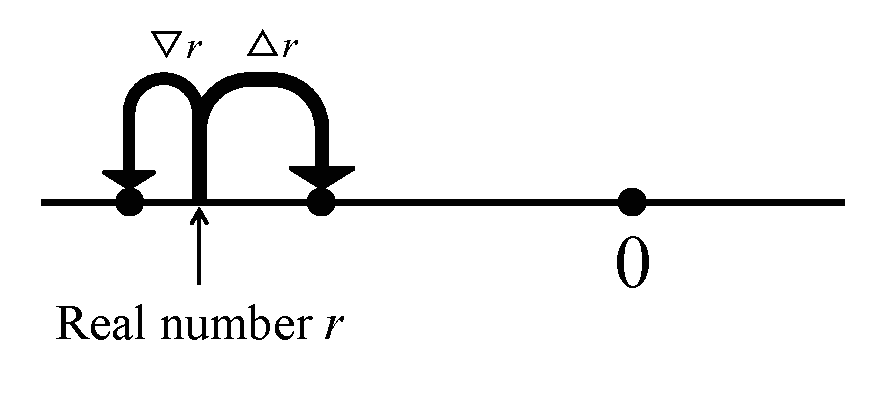
\includegraphics[width=58mm]{figs/3_minus.eps}
% \end{center}
%  \end{minipage}
% \begin{minipage}{0.4\hsize}
% \begin{center}
%  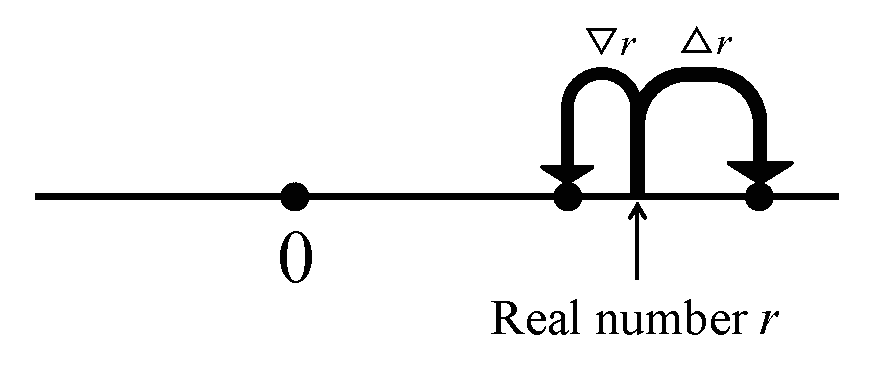
\includegraphics[width=58mm]{figs/3_plus.eps}
% \end{center}
%  \end{minipage}
%   \caption{Rounding ($\cdot$ is a floating-point number).}
% \label{3:fig_plus_minus}
%\end{figure}

%
%----------------------------------------------------------------------------------------------------------------------------------------------
%\subsection{浮動小数点演算の正規化数}

%
%----------------------------------------------------------------------------------------------------------------------------------------------
%\subsection{浮動小数点演算の非正規化数}

%
%----------------------------------------------------------------------------------------------------------------------------------------------
%\subsection{浮動小数点演算のアンダーフローとオーバーフロー}

%
%
%----------------------------------------------------------------------------------------------------------------------------------------------
%----------------------------------------------------------------------------------------------------------------------------------------------
%----------------------------------------------------------------------------------------------------------------------------------------------
\section{1回の浮動小数点数同士の演算における品質保証}
ここでは1回の浮動小数点数同士の演算における結果の品質保証法を紹介します．
具体的には，$a, b \in {\mathbb F}$，すなわち，$a$も$b$も誤差なく浮動小数点数で記述されているとしたときの四則演算($a+b$, $a-b$, $a*b$, $a/b$)の品質保証について取り上げます．

品質の保証を行う際の信念は，「1 bitたりともさぼらずに必ず数学的に正しい結果」を返すことです．
しかしながら，$a+b$という結果は多くの場合，実数${\mathbb R}$になってしまいコンピュータでは表現できません．
そこで，コンピュータで表現できる$a+b$で表せる数学的に正しい結果は，2つの浮動小数点数$c_l, c_u \in {\mathbb F}$を用いて
\begin{align*}
	c_l \le a + b \le c_u
\end{align*}
のように結果を挟み込むことです．
別の言い方をすれば，「区間$[c_l, c_u]$の中に$a + b$の結果が含まれている」あるいは「$a + b \in [c_l, c_u]$」といえます．
もちろん$c_l$と$c_u$の幅が大きければ，使い物にならない結果かもしれません．

では，次に$c_l$と$c_u$をどのように作ればよいか，考えてみましょう．
まず，演算子$+$を用いて丸めも含めた演算をもう一度おさらいすると
\begin{align*}
 a + b \in {\mathbb R}&: ~ \mbox{数学における足し算．結果は浮動小数点数とは限らない} \\
 a ~ \tilde{+} ~ b \in {\mathbb F}&: ~ \mbox{$a+b$に最も近い浮動小数点数．} \\
 a ~ \overline{+} ~ b \in {\mathbb F}&: ~ \mbox{$a+b$よりも大きい浮動小数点数のうち最も小さい数．}\\
 a ~ \underline{+} ~ b \in {\mathbb F}&: ~ \mbox{$a+b$よりも小さい浮動小数点数のうち最も大きい数．}
\end{align*}
でした．
IEEE 754 標準では，$+$以外にも$-, *, /$と$\sqrt{\cdot}$のみ丸めモードの変更による動作の保証がされておりましたね．
よって，$c_l = a ~ \underline{+} ~ b$, $c_u = a ~ \overline{+} ~ b$とすれば，
\begin{align*}
	a + b \in [ a ~ \underline{+} ~ b, a ~ \overline{+} ~ b  ] = \{ c \in {\mathbb R} ~ | ~  a ~ \underline{+} ~ b \le c \le a ~ \overline{+} ~ b \}
\end{align*}
となり，$a + b$の真の結果はわからないですが，コンピュータで数学的に正しい結果$[ a ~ \underline{+} ~ b, a ~ \overline{+} ~ b  ]$を得ることができます．

同様に他の四則演算についても
\begin{align*}
	a - b &\in [ a ~ \underline{-} ~ b, a ~ \overline{-} ~ b  ] \\
	a \cdot b &\in [ a ~ \underline{\cdot} ~ b, a ~ \overline{\cdot} ~ b  ] \\
	a / b &\in [ a ~ \underline{/} ~ b, a ~ \overline{/} ~ b  ]
\end{align*}
のように2つの浮動小数点数の丸めモードを用いて真の結果を含む区間を得ることができます．

\Mondai
プログラム
\begin{verbatim}
   #include <stdio.h>
   #include <math.h>
	
   int main(void){
     double a = 0.1;
     double b = 1.1;
     double c;

     c = a + b;
  
     printf("%lf\n", c);
   }
\end{verbatim}
の$a$と$b$を品質保証を行う計算に変えよ($c$については次節で取り扱う)．
ただし，丸めモードは以下のような fenv.h を使用すること:
\begin{verbatim}
	#include <fenv.h>
	#include <math.h>

	fesetround(FE_UPWARD);    // 上向き丸めモードへ変更
	fesetround(FE_DOWNWARD);  // 下向き丸めモードへ変更
	fesetround(FE_TONEAREST); // 最近点丸めモードへ変更
\end{verbatim}

\vspace{5mm}

\Kaitourei
$0.1$と書いてしまうと誤差が発生するために，$1.0/10.0$のように倍精度浮動小数点数で誤差なく記述できる値の計算に変形してから，丸めモードを用いて上端と下端を計算すればよい ($1.1$についても同様である)．
具体的には以下のようなプログラムになる．
\begin{verbatim}
   #include <stdio.h>
   #include <fenv.h>
   #include <math.h>
	
   int main(void){

     fesetround(FE_DOWNWARD);
       double al = 1.0/10.0;    // 下向き丸めで1/10を計算
     fesetround(FE_UPWARD);
       double au = 1.0/10.0;    // 上向き丸めで1/10を計算

     fesetround(FE_DOWNWARD);
       double bl = 11.0/10.0;    // 下向き丸めで11/10を計算
     fesetround(FE_UPWARD);
       double bu = 11.0/10.0;    // 上向き丸めで11/10を計算

     double c;
     c = a + b;  // ここはどうする?っていうのが次の話!

     printf("%lf\n", c);
   }
\end{verbatim}



上記の解答を見てみると，それぞれ$0.1 \in [a_l, a_u]$, $1.1 \in [b_l, b_u]$となる区間が得られます．
ただし，よく見ると同じ計算(例えば$1.0/10.0$)が出てきます．
もちろん，丸めモードを変えているので，結果は変わります．
しかし，プログラムにはコンパイラの最適化オプションによっては，賢いコンパイラによって$1.0/10.0$は同じ計算だとみなされてしまい
\begin{verbatim}
     fesetround(FE_DOWNWARD);
       double al = 1.0/10.0;    // 下向き丸めで1/10を計算
     fesetround(FE_UPWARD);
       double au = al;

     fesetround(FE_DOWNWARD);
       double bl = 11.0/10.0;    // 下向き丸めで11/10を計算
     fesetround(FE_UPWARD);
       double bu = bl;
\end{verbatim}
のように意図とは違うプログラムに置き換えてしまうかもしれませんので，注意してください．


%
%----------------------------------------------------------------------------------------------------------------------------------------------
%----------------------------------------------------------------------------------------------------------------------------------------------
%----------------------------------------------------------------------------------------------------------------------------------------------
\section{上端下端型の区間演算} \label{intval}
前節の問題の解答例では,$a = 0.1 \in[a_l, a_u]$, $b = 1.1 \in [b_l, b_u]$のように端点が浮動小数点数となる区間を用いて，$0.1$や$1.1$をコンピュータで数学的に正しく保持しました．
しかし，その先のプログラムでは$c = a + b$を計算しています．
このままでは，区間同士の$+$の意味や規則がわからないため，コンパイルエラーになってしまいます．
本節では，区間同士の四則演算を定義することで，演算結果の品質を保証することが目標です．

まず，丸め誤差が入らない状況における区間同士の演算を考えています．
$a \in[a_l, a_u]$, $b \in [b_l, b_u]$としたときの$a + b$の結果は集合
\begin{align*}
	\{ a + b \in {\mathbb R} ~ | ~ \forall a \in [a_l, a_u], ~ \forall b \in [b_l, b_u] \}
\end{align*}
で表されます．
もちろん足し算以外の四則演算($-, \cdot, /$)でも同じです．
例えば，$a = 0.1 \in[a_l, a_u]$, $b = 1.1 \in [b_l, b_u]$のとき，$a + b = 1.2$は
\begin{align*}
	1.2 \in \{ a + b \in {\mathbb R} ~ | ~ \forall a \in [a_l, a_u], ~ \forall b \in [b_l, b_u] \}
\end{align*}
のように集合内に元の足し算結果が必ず含まれます．
すなわち，この右辺の集合を区間同士の演算結果として考えれば，数学的に正しい結果を得ることが可能です．
すなわち，区間同士の四則演算は
\begin{align*}
	[a_l, a_u] + [b_l, b_u] =& \{ a + b \in {\mathbb R} ~ | ~  \forall a \in [a_l, a_u], ~ \forall b \in [b_l, b_u]  \} \\
	[a_l, a_u] - [b_l, b_u] =& \{ a - b \in {\mathbb R} ~ | ~  \forall a \in [a_l, a_u], ~ \forall b \in [b_l, b_u]  \} \\
	[a_l, a_u] \cdot [b_l, b_u] =& \{ a \cdot b \in {\mathbb R} ~ | ~  \forall a \in [a_l, a_u], ~ \forall b \in [b_l, b_u]  \} \\
	[a_l, a_u] / [b_l, b_u] =& \{ a / b \in {\mathbb R} ~ | ~  \forall a \in [a_l, a_u], ~ \forall b \in [b_l, b_u]  \}
\end{align*}
のように定義します．
そのうえで，右辺の集合は閉区間になり，端点$a_l, a_u, b_l, b_u \in {\mathbb R}$のみで書き表せることが知られています:
\begin{itemize}
	\item 加算：$ \{ a + b ~ | ~a \in [a_l, a_u], b \in [b_l, b_u] \} = [a_l + b_l, \ a_u + b_u]$
	\item 減算：$ \{ a - b ~ | ~a \in [a_l, a_u], b \in [b_l, b_u] \} = [a_l - b_u,\ a_u - b_l]$
	
	\item 乗算：$ \{ a \cdot b ~ | ~a \in [a_l, a_u], b \in [b_l, b_u] \} = $\\
	$ ~~~~~~~~~ [\min \{ a_l \cdot b_l, ~ a_u \cdot b_l, ~ a_l \cdot b_u, ~ a_u \cdot b_u \}, ~ \max \{ a_l \cdot b_l, ~ a_u \cdot b_l, ~ a_l \cdot b_u, ~ a_u \cdot b_u \} ]$
	\item 除算：$ \{ a / b ~ | ~a \in [a_l, a_u], b \in [b_l, b_u] \} = $\\
	$ ~~~~~~~~~ [\min \{ a_l / b_l, ~ a_u / b_l, ~ a_l / b_u, ~ a_u / b_u \}, ~ \max \{ a_l / b_l, ~ a_u / b_l, ~ a_l / b_u, ~ a_u / b_u \} ]$\\
	$ ~~~~~~~~~ $ただし$0 \notin [b_l,\ b_u]$
\end{itemize}
この演算で計算した区間の中には，真の答えが必ず含まれています．




しかし，この区間の端点も浮動小数点数で表さなければコンピュータで取り扱うことができません．
注意していただきたい点は，端点$a_l, a_u, b_l, b_u$は，既に浮動小数点数として計算機で保持できていることが前提です．
演算前の端点$a_l, a_u, b_l, b_u$が浮動小数点数でない場合，演算以前に品質保証の取り扱いにミスがあるので注意してください．
ここで気にしなければならない誤差は，演算結果を構成する端点$a_l, a_u, b_l, b_u \in {\mathbb F}$同士の演算(例えば，$a_l + b_l$など)の誤差です．
例えば，$a_l, a_u, b_l, b_u \in {\mathbb F}$における足し算では
\begin{align*}
	[a_l, a_u] + [b_l, b_u] = [a_l + b_l, \ a_u + b_u] \subset& [a_l ~ \underline{+} ~ b_l, \ a_u ~ \overline{+} ~ b_u]
\end{align*}
のように，丸めモードの変更を変更することで，真の像を包含するような区間を作成します．
ここでは，丸めモードまで含めた演算規則として，以下のような機械区間演算を定義します:

\begin{defi}[機械区間演算]\label{def:round_interval}
$a_l, a_u, b_l, b_u \in {\mathbb F}$としたとき，以下として機械区間演算を定義する:
\begin{itemize}
	\item 加算：$[a_l,\ a_u]+[b_l,\ b_u] = [a_l ~ \underline{+} ~ b_l,\ a_u ~ \overline{+} ~ b_u]$
	\item 減算：$[a_l,\ a_u]-[b_l,\ b_u] = [a_l ~ \underline{-} ~ b_u,\ a_u ~ \overline{-} ~ b_l]$
	
	\item 乗算：$ [a_l,\ a_u]\times[b_l,\ b_u] = $\\
	$ ~~~~~~~~~ [\min \{ a_l ~ \underline{\cdot} ~ b_l, a_u ~ \underline{\cdot} ~ b_l, a_l ~ \underline{\cdot} ~ b_u,\ a_u ~ \underline{\cdot} ~ b_u \}, \max \{ a_l ~ \overline{\cdot} ~ b_l, a_u ~ \overline{\cdot} ~ b_l, a_l ~ \overline{\cdot} ~ b_u, a_u ~ \overline{\cdot} ~ b_u \}]$
	\item 除算：$ [a_l,\ a_u]/[b_l,\ b_u]= $\\
	$ ~~~~~~~~~ [\min \{ a_l ~ \underline{/} ~ b_l, a_u ~ \underline{/} ~ b_l, a_l ~ \underline{/} ~ b_u,\ a_u ~ \underline{/} ~ b_u \}, \max \{ a_l ~ \overline{/} ~ b_l, a_u ~ \overline{/} ~ b_l, a_l ~ \overline{/} ~ b_u, a_u ~ \overline{/} ~ b_u \}]$\\
	$ ~~~~~~~~~ $ただし$0 \notin [b_l,\ b_u]$
\end{itemize}
\end{defi}

\Mondai
プログラム
\begin{verbatim}
   #include <stdio.h>
   #include <math.h>
	
   int main(void){
     double a = 0.1;
     double b = 1.1;
     double c;

     c = a + b;
  
     printf("%lf\n", c);
   }
\end{verbatim}
の$a$と$b$及び，$c = a + b$の品質保証を行う計算に変えよ．
ただし，丸めモードは以下のような fenv.h を使用すること:
\begin{verbatim}
	#include <fenv.h>

	fesetround(FE_UPWARD);    // 上向き丸めモードへ変更
	fesetround(FE_DOWNWARD);  // 下向き丸めモードへ変更
	fesetround(FE_TONEAREST); // 最近点丸めモードへ変更
\end{verbatim}

\vspace{5mm}

\Kaitourei
$a$と$b$の保証については前節に取り上げてあることに注意し解答を示す:
\begin{verbatim}
   #include <stdio.h>
   #include <fenv.h>
   #include <math.h>
	
   int main(void){

     fesetround(FE_DOWNWARD);
       double al = 1.0/10.0;    // 下向き丸めで1/10を計算
     fesetround(FE_UPWARD);
       double au = 1.0/10.0;    // 上向き丸めで1/10を計算

     fesetround(FE_DOWNWARD);
       double bl = 11.0/10.0;    // 下向き丸めで11/10を計算
     fesetround(FE_UPWARD);
       double bu = 11.0/10.0;    // 上向き丸めで11/10を計算

     fesetround(FE_TONEAREST);  // 最近点丸めにもどす

     double cl, cu;
     fesetround(FE_DOWNWARD);
       cl = al + bl;
     fesetround(FE_UPWARD);
       cu = au + bu;

     fesetround(FE_TONEAREST);  // 最近点丸めにもどす

     printf("%lf\n", cl);
     printf("%lf\n", cu);
   }
\end{verbatim}

\vspace{5mm}


以下の問題は，ベクトル，行列を扱う際に良く使う演算です．
場合によっては，計算途中の結果を区間として保持する必要がなく，一気に計算可能な例があります．
どのような演算が一気に計算可能な例になるか覚えておきましょう．

\vspace{5mm}

\Mondai
$a, b, c, c_l, c_u \in {\mathbb F}$とする．
そのとき，以下の結果を包含する両端点に浮動小数点数を持つ区間を，丸めモード変更付きの四則演算を用いて作成せよ:
\begin{align*}
	\mbox{(1)}& ~ a \cdot b - c \\
	\mbox{(2)}& ~c - a \cdot b \\
	\mbox{(3)}& ~a \cdot b + [ c_l, c_u ]
\end{align*}

\vspace{5mm}

\Kaitourei
\noindent\textbf{(1)}:
\begin{align*}
	a \cdot b - c \subset& [ a ~ \underline{\cdot} ~ b, ~ a ~ \overline{\cdot} ~ b  ] - c \\
	=& [ a ~ \underline{\cdot} ~ b, ~ a ~ \overline{\cdot} ~ b  ] - [c, c] \\
	\subset&  [ a ~ \underline{\cdot} ~ b ~ \underline{-} ~ c , ~ a ~ \overline{\cdot} ~ b ~ \overline{-} ~ c  ]
\end{align*}
注意点としては，$[ a ~ \underline{\cdot} ~ b, ~ a ~ \overline{\cdot} ~ b  ] - c$は$[ a ~ \underline{\cdot} ~ b, ~ a ~ \overline{\cdot} ~ b  ] - [c, c]$のように$c$を点区間として計算すればよい．
上記の計算により，
\begin{verbatim}
     fesetround(FE_DOWNWARD);
       res_lower = a*b - c;
     fesetround(FE_UPWARD);
       res_upper = a*b - c;
\end{verbatim}
のように途中結果を区間として保持せずに区間を作成できる．

\medskip\noindent\textbf{(2)}:
\begin{align*}
	c - a \cdot b \subset& c - [ a ~ \underline{\cdot} ~ b, ~ a ~ \overline{\cdot} ~ b  ]  \\
        \subset& [c, c] - [ a ~ \underline{\cdot} ~ b, ~ a ~ \overline{\cdot} ~ b  ]  \\
	\subset&  [ c ~ \underline{-} ~ a ~ \overline{\cdot} ~ b , ~ c ~ \overline{-} ~a ~ \underline{\cdot} ~ b  ]
\end{align*}
上記の計算により，
\begin{verbatim}
     fesetround(FE_DOWNWARD);
       tmp_lower = a*b;
     fesetround(FE_UPWARD);
       tmp_upper = a*b;
       res_upper = c - tmp_lower;
     fesetround(FE_DOWNWARD);
       res_lower = c - tmp_upper;
\end{verbatim}
のように$a \cdot b$の結果を区間として保持しなければならない．

初めて扱った人がしがちなミスとして
\begin{verbatim}
     誤ったプログラム:
     fesetround(FE_DOWNWARD);
       res_lower = c - a*b;
     fesetround(FE_UPWARD);
       res_upper = c - a*b;
\end{verbatim}
としてしまいます．
これでは，数学的に正しくない結果を返しているので注意してください．

\medskip\noindent\textbf{(3)}:
\begin{align*}
	a \cdot b + [ c_l, c_u ] \subset& [ a ~ \underline{\cdot} ~ b, ~ a ~ \overline{\cdot} ~ b  ] + [ c_l, c_u ] \\
	\subset& [ a ~ \underline{\cdot} ~ b ~ \underline{+} ~ c_l , ~ a ~ \overline{\cdot} ~ b ~ \overline{+} ~ c_u  ]
\end{align*}
上記の計算により，
\begin{verbatim}
     fesetround(FE_DOWNWARD);
       res_lower = a*b + cl;
     fesetround(FE_UPWARD);
       res_upper = a*b + cu;
\end{verbatim}
のように$a \cdot b$の結果を保持せずに区間を作成できる．
この結果から浮動小数点数の$n$次元ベクトル$a \in {\mathbb F}^n$と$b \in {\mathbb F}^n$の内積$a \cdot b$は区間
\begin{align}\label{eq:inner_def}
	[ a_1 \underline{\cdot} b_1 \underline{+} a_2 \underline{\cdot} b_2 \underline{+} \cdots \underline{+}  a_n \underline{\cdot} b_n, ~~ a_1 \overline{\cdot} b_1 \overline{+} a_2 \overline{\cdot} b_2 \overline{+} \cdots \overline{+}  a_n \overline{\cdot} b_n ]
\end{align}
として得られるため，
\begin{verbatim}
     fesetround(FE_DOWNWARD);
       for (int i = 0; i < n; i++)
         res_lower += a[i]*b[i];
     fesetround(FE_UPWARD);
       for (int i = 0; i < n; i++)
         res_upper += a[i]*b[i];
\end{verbatim}
のように計算できる．
この例のように「一気に計算する技を利用できるのはあくまで数学的に正しい状況のみ」で，基本は「機械区間演算」であることに注意してください．

%
%----------------------------------------------------------------------------------------------------------------------------------------------
%----------------------------------------------------------------------------------------------------------------------------------------------
%----------------------------------------------------------------------------------------------------------------------------------------------
\section{浮動小数点数で成分を持つ点行列同士の行列積}
前節の\eqref{eq:inner_def}の結果をまとめると浮動小数点数で成分を持つベクトルの内積は次のようなことが言えます:

\begin{Thm}[浮動小数点数における内積の包含] \label{thm:float_inner}
	浮動小数点数の$n$次元のベクトル$a \in {\mathbb F}^n$と$b \in {\mathbb F}^n$は
	\begin{align*}
		a \cdot b \subset [ a ~ \underline{\cdot} ~ b , a ~ \overline{\cdot} ~ b ]
	\end{align*}
	となる．
	ただし，$a \underline{\cdot} b$は内積の演算をすべて下向き丸めで計算し，$a \overline{\cdot} b$は内積の演算をすべて上向き丸めで計算することを意味し，\eqref{eq:inner_def}のように計算していることを前提とする．
\end{Thm}

もちろん，同じように行列積についても以下のことがいえます:
\begin{Thm}[浮動小数点数における行列積の包含] \label{thm:float_matmul}
	浮動小数点数の行列$A \in {\mathbb F}^{l \times m}$と$B \in {\mathbb F}^{m \times n}$は
	\begin{align*}
		A \cdot B \subset [ A ~ \underline{\cdot} ~ B , A ~ \overline{\cdot} ~ B ]
	\end{align*}
	となる．
	ただし，$A \underline{\cdot} B$は行列積の演算をすべて下向き丸めで計算し，$a \overline{\cdot} b$は行列積の演算をすべて上向き丸めで計算することを意味し，各成分ごとで現れる内積は\eqref{eq:inner_def}のように計算していることを前提とする．
\end{Thm}

最後の注意書きは，行列積を工夫するアルゴリズムStrassenなどでは引き算が含まれるため，上記の定理の範囲外になってしまいますので注意してください．
例えば，$A,\ B\in\F^{n\times n}$としたときの行列積は以下のように計算できます:

\begin{verbatim}
	#include <fenv.h>
	fesetround(FE_UPWARD);   //上向き丸めモードへ変更
	C_u=A*B;                 //上向き丸めで行列積
	fesetround(FE_DOWNWARD); //下向き丸めモードへ変更
	C_d=A*B;                 //下向き丸めで行列積
\end{verbatim}

行列積$A*B$に最適化されたBLAS(例えばdgemmなど)を用いることで非常に高速に点行列同士の積の包含を得ることができます．
ただし，例えば3つの行列の積$A*B*C$などの一般的な場合は区間行列の演算になるため結果の包含は単純には得られないので注意してください．
区間同士の行列積については\ref{chap:basic_matrix}章で取り上げます．

また，注意点としては，$A*B$を演算する前に丸めモードを変更していますが，行列演算に利用する全ノード・全スレッドの丸めモードが変更されている必要があります．
そのため，BLASなどの高速ルーチンを利用する際には全ノード・全スレッドの丸めモードが変更されている保証が必要になります．


%
%----------------------------------------------------------------------------------------------------------------------------------------------
%----------------------------------------------------------------------------------------------------------------------------------------------
%----------------------------------------------------------------------------------------------------------------------------------------------
\section{区間演算の落とし穴}
区間演算を初めて勉強したとき著者は「すべて区間演算で計算すればいいんじゃない?」って思いました．
しかし，残念ながら世の中そんなにうまい話はなく，「区間演算を繰り返すことによる過大評価」という最大の欠点があります．
そのために，現在では，「最初に近似解を求めてから，その結果の品質を保証する際に区間演算を使う」という検算手法として区間演算は利用されます．
連立一次方程式を例にとると，(1) Gaussの消去法は通常の浮動小数点数の演算で行い近似解を得る，(2) そのうえで，得られた近似解と真の解の誤差を計算する際に区間演算で数学的に正しい結果で証明，のような流れです．

ここでは，欠点となる例をいくつか紹介したいと思います．
まず，$x^2, x \in [-1, 1]$について取り扱いたいと思います．
$x^2 = x \cdot x$だからといって演算を行うと
\begin{align*}
	[-1, 1] \cdot [-1, 1] = [-1, 1]
\end{align*}
となります．
もちろん，この結果は数学的には正しいです．
しかし，よく考えると$0 \le x^2, \forall x \in {\mathbb R}$ですので，負の値が区間に含まれてしまう結果は良い結果とは言えません．
この原因は，区間演算の定義に立ち戻ると
\begin{align*}
	[-1, 1] \cdot [-1, 1] = \{ x \cdot y ~ | ~ x \in [-1, 1], ~ y \in [-1, 1]  \}
\end{align*}
となり，$x$と$y$は独立した変数としてみなしているため$x = 1, y = -1$のような状況が発生し，負の値が生まれます．
本来は$x^2$の像は
\begin{align*}
	[-1, 1]^2 = \{ x^2 = x \cdot x ~ | ~ x \in [-1, 1]  \}
\end{align*}
となるため，$x \cdot y$のように独立には動かず
\begin{align*}
	[-1, 1]^2 = [0, 1]
\end{align*}
のようになります．
あくまで区間演算は2つの区間に依存関係がない独立した変数としての結果となるため，依存関係がある演算を行う場合には過大評価になってしまいます．

同じように，$x \in [-1, 1]$に対して，
\begin{align*}
	x - x = [-1, 1] - [-1, 1] = [-2, 2] = \{ x - y ~ | ~ \forall x \in [-1, 1], ~ \forall y \in [-1, 1]  \}
\end{align*}
となってしまうため，過大評価になってしまいます(実際は$\{ x - x = 0 ~ | ~ \forall x \in [-1, 1]  \}$)．
$x^2$や$x - x$のようにわかりきった計算の場合は，専用の演算をプログラムすればよいですが，例えば漸化式
\begin{align*}
	x_0 \in& [ x_l, x_u ] \\
	x_1 \in& [ y_l, y_u ] \\
	x_{n} =& f(x_{n-1}, x_{n - 2})
\end{align*}
のように依存関係がわかりにくくなってしまう演算は非常に多くあります．
解消法としては，平均値形式やアフィン演算などがありますが，本書では取り扱いません．


次の例として回転行列
\begin{align*}
	A(\theta) = \left( \begin{array}{cc}
	\cos(\theta) & -\sin(\theta) \\
	\sin(\theta) & \cos(\theta)
	\end{array}\right),
\end{align*}
と区間ベクトル
\begin{align*}
	x = \left( \begin{array}{c}
	x_1 \\
	x_2
	\end{array}\right) = \left(
	\begin{array}{c}
	\mbox{[-1, 1]} \\
	\mbox{[-1, 1]}
	\end{array}
	\right).
\end{align*}
について考えてみます．
$x$を図で書いてみると図 \ref{3:wrap1}のようになります．

\begin{figure}[htb]
 \begin{center}
  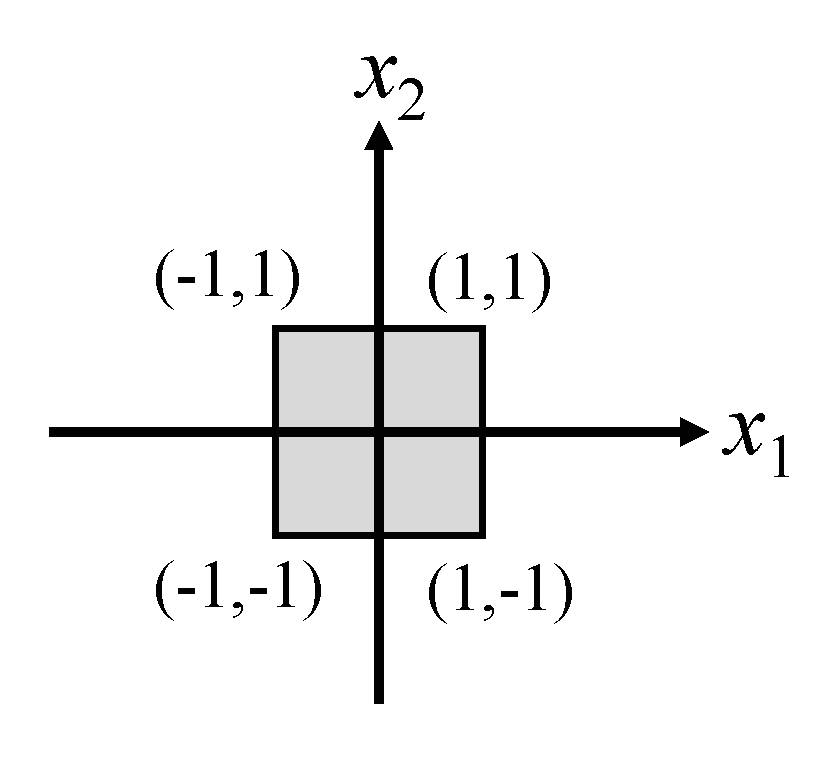
\includegraphics[width=50mm]{figs/wrapping_effect1.eps}
 \end{center}
  \caption{Wrapping effect1}
 \label{3:wrap1}
\end{figure}

$\pi/4$だけ$x$を回転を意味する$A(\pi/4)x$の像は図 \ref{3:wrap2}のようになります．
しかしながら，区間演算を用いて計算すると
\begin{align*}
	A(\pi/4)x = \left( \begin{array}{cc}
	\frac{\sqrt{2}}{2} & -\frac{\sqrt{2} }{2} \\
	\frac{\sqrt{2} }{2} & \frac{\sqrt{2} }{2}
	\end{array}\right)\left(
	\begin{array}{c}
	\mbox{[-1, 1]} \\
	\mbox{[-1, 1]}
	\end{array}
	\right) = \left(
	\begin{array}{c}
	\mbox{[}-\sqrt{2}, \sqrt{2}\mbox{]} \\
	\mbox{[}-\sqrt{2}, \sqrt{2}\mbox{]}
	\end{array}
	\right),
\end{align*}
のようになり，図で表すと図 \ref{3:wrap3}のオレンジ色の部分になります．
図を見てもわかるように，区間演算はそれぞれの軸に対して区間を作成するために，2次元ベクトル以上の場合は表現できる集合が非常に限定されてしまいます．

\begin{figure}[htb]
 \begin{center}
  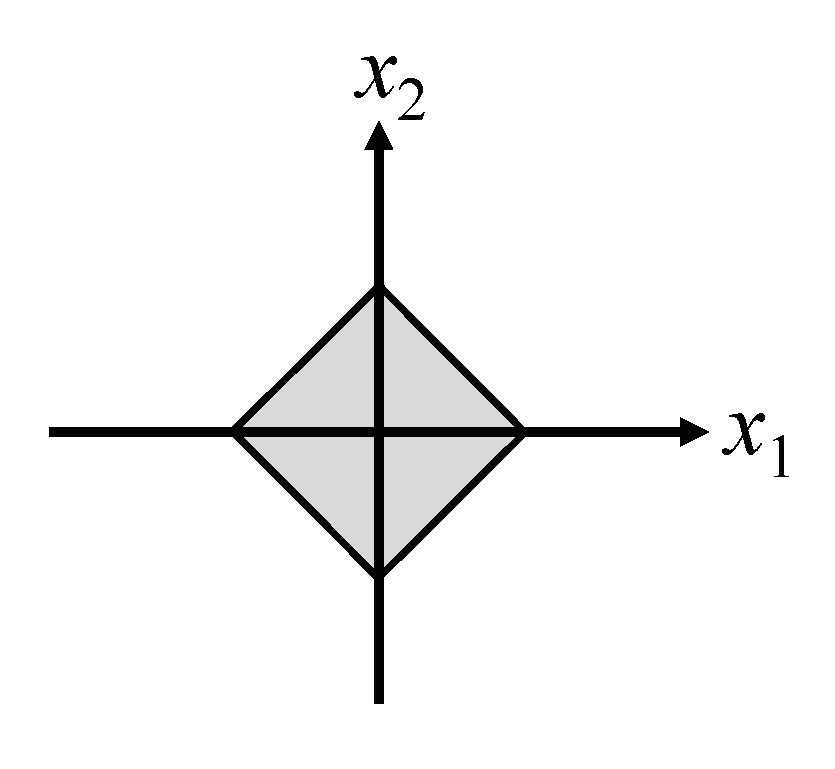
\includegraphics[width=50mm]{figs/wrapping_effect2.eps}
 \end{center}
  \caption{Wrapping effect2}
 \label{3:wrap2}
\end{figure}

\begin{figure}[htb]
 \begin{center}
  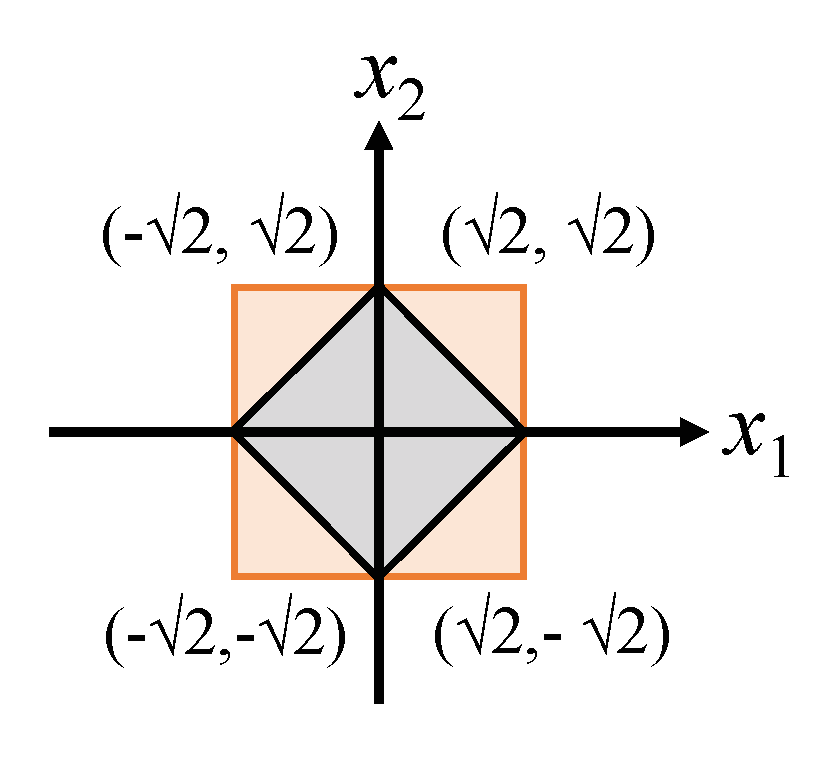
\includegraphics[width=50mm]{figs/wrapping_effect3.eps}
 \end{center}
  \caption{Wrapping effect3}
 \label{3:wrap3}
\end{figure}

さらに，もう一度，$\pi/4$だけ回転させる，すなわち$A(\pi/4) \left( A(\pi/4)x \right)$とすると真の像は図 \ref{3:wrap2}に戻ります．
しかしながら，区間演算では
\begin{align*}
A\left( \frac{\pi}{4} \right) \left( A\left( \frac{\pi}{4} \right)x \right) = \left(
\begin{array}{c}
\mbox{[}-2, 2\mbox{]} \\
\mbox{[}-2, 2\mbox{]}
\end{array}
\right)
\end{align*}
から図 \ref{3:wrap4}のようになり，非常に過大評価になってしまうことがわかります．

\begin{figure}[htb]
 \begin{center}
  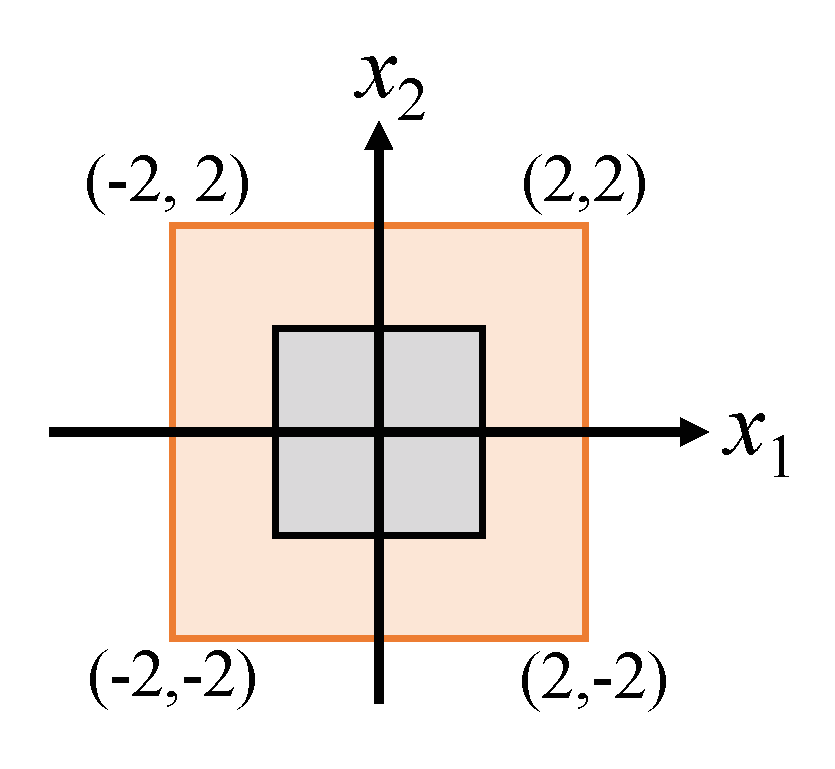
\includegraphics[width=50mm]{figs/wrapping_effect4.eps}
 \end{center}
  \caption{Wrapping effect4}
 \label{3:wrap4}
\end{figure}

このような影響はラッピングエフェクトと呼ばれます．
そのために，区間演算はできる限り後に行ったほうがよいです．
例えば，計算順序をかえると
\begin{align*}
\left( A\left( \frac{\pi}{4} \right) A\left( \frac{\pi}{4} \right) \right) x  = \left( \begin{array}{cc}
0 & -1 \\
1 & 0
\end{array}\right)\left(
\begin{array}{c}
\mbox{[-1, 1]} \\
\mbox{[-1, 1]}
\end{array}
\right) = \left(
\begin{array}{c}
\mbox{[}-1, 1 \mbox{]} \\
\mbox{[}-1, 1 \mbox{]}
\end{array}
\right).
\end{align*}
となることから，精度の良い結果を得ることができます．



%
%----------------------------------------------------------------------------------------------------------------------------------------------
%----------------------------------------------------------------------------------------------------------------------------------------------
%----------------------------------------------------------------------------------------------------------------------------------------------
\section{中心半径型の区間と区間演算}\label{sec:midrad_op}
今まで扱ってきた区間$[a_l, a_u] = \{ a \in {\mathbb R} ~ | ~ a_l \le a \le a_u \}$は，上端と下端から表現される区間であるため，ここでは上端下端型の区間と呼びます．
それに対し，中心$a_m \in {\mathbb R}$と半径$a_r \ge 0$を用いても区間
\begin{align*}
	\langle a_m, a_r  \rangle := \{ a \in {\mathbb R} ~ | ~ | a - a_m | \le a_r  \}
\end{align*}
を表現することができ，こちらを中心半径型の区間と呼びます．
本節の目標は，中心半径型の区間を利用することで，過大評価にはなるかわりに最大値/最小値の判別が必要ない計算方法を紹介します．
この方法を拡張することで，区間同士の行列積に適用することができます．
そのうえ，行列積に対し，BLASなどの既存の高速に最適化されたプログラムを利用した高速な品質保証法を実現できます．


まず，上端下端型の区間と中心半径型の区間の関係性は
\begin{align*}
	[ a_l, a_u ] = \left\langle \frac{ a_l + a_u }{2}, ~ \frac{ a_u - a_l }{2}  \right\rangle
\end{align*}
であり，
\begin{align*}
	\langle a_m, a_r  \rangle = [ a_m - a_r, ~ a_m + a_r ]
\end{align*}
となります．
しかしながら，浮動小数点数同士の演算は一般的には浮動小数点数になるとは限らないため，「上端下端型から中心半径型への変換」および「中心半径型から上端下端型への変換」をコンピュータで行う際には誤差が生じます．
そのために，双方の変換でも丸めモードの変更を行い元の区間を包含する区間を作成します．

まず，「コンピュータを用いた中心半径型から上端下端型への変換」は単純であり，$a_m, a_r \in {\mathbb F}$とすると
\begin{align*}
	\langle a_m, a_r  \rangle \subset [ a_m ~ \underline{-} ~ a_r, ~ a_m ~  \overline{+} ~ a_r ]
\end{align*}
として変換することができます．
それに対し，「コンピュータを用いた上端下端型から中心半径型への変換」は中心の演算に対し，どうすれば良いか考えなければなりません．


\begin{Thm}[上端下端型から中心半径型への変換]\label{thm:infsup_to_midrad}
	${\mathbb F}$を基数$2$の浮動小数点数とし，$a_l, a_u \in {\mathbb F}$が$a_l \le a_u$を満たすとする．	  
	そのとき，$a_m, a_r \in {\mathbb F}$を
	\begin{align*}
		a_m = (a_l ~ \overline{+} ~ a_u) \overline{/} 2 , ~ a_r = a_m ~ \overline{-} ~ a_l
	\end{align*}
	とすると，
	\begin{align*}
		[ a_l, a_u ] \subset \langle a_m, a_r \rangle
	\end{align*}
	となる．
\end{Thm}

\begin{Proof}
	$a_m - a_r \le a_l$と$a_u \le a_m + a_r$を示せばよい．

	まず，$a_m - a_r \le a_l$から示す．
	丸めモードの定義から$a_m ~ \overline{-} ~ a_l \ge a_m - a_l$となることに注意すると
	\begin{align*}
		a_l + a_r =a_l + (  a_m ~ \overline{-} ~ a_l ) \ge a_l + (  a_m - a_l ) = a_m
	\end{align*}
	となる．
	よって，上式から$a_r$を引くと$a_l \ge a_m - a_r$になる．

	次に，$a_u \le a_m + a_r$を示す．
	まず，$a_l ~ \overline{+} ~ a_u$の結果は基数$2$の浮動小数点数になる．
	そのうえで，基数$2$の浮動小数点数に対し，(どのような丸めモードでも)$2$を割っても誤差は生じないため，
	\begin{align*}
		(a_l ~ \overline{+} ~ a_u) \overline{/} 2 = (a_l ~ \overline{+} ~ a_u)/2
	\end{align*}
	となる．
	そのうえで，丸めモードの定義から$a_l ~ \overline{+} ~ a_u \ge a_l + a_u$となることに注意すると
	\begin{align*}
		a_m + a_r =& ( (a_l ~ \overline{+} ~ a_u) \overline{/} 2 ) + (a_m ~ \overline{-} ~ a_l) = \left( \frac{a_l ~ \overline{+} ~ a_u}{2} \right) + (a_m ~ \overline{-} ~ a_l) \\
		\ge& \frac{a_l + a_u}{2} + a_m - a_l = \frac{a_l + a_u}{2}  + \left( ( (a_l ~ \overline{+} ~ a_u) \overline{/} 2 \right) - a_l \\
		\ge& \frac{a_l + a_u}{2}  +  \frac{a_l + a_u}{2} - a_l = a_l + a_u - a_l = a_u
	\end{align*}

\qed
\end{Proof}

次に，中心半径型における演算規則を紹介します．
足し算と引き算は
\begin{align*}
	\langle a_m, a_r  \rangle \pm \langle b_m, b_r  \rangle =& [ a_m - a_r, ~ a_m + a_r ] \pm [ b_m - b_r, ~ b_m + b_r ] \\
	=& [a_m \pm b_m - a_r - b_r, ~ a_m \pm b_m + a_r + b_r] \\
	=&  \left\langle a_m \pm b_m, ~ a_r + b_r  \right\rangle
\end{align*}
と簡単に得られます(が，わざわざ中心半径型で行うメリットはありません...)．

それに対し，掛け算は工夫が必要であり，中心半径型で計算するメリット(とデメリット)があります．

\begin{Thm}[中心半径型の区間の積] \label{thm:midrad_mul}
	$a_m,  b_m \in {\mathbb R}$と非負の実数$a_r, b_r \in {\mathbb R}$とする．	  
	そのとき，中心半径型の区間の積は
	\begin{align*}
		\langle a_m, a_r \rangle \cdot \langle b_m, b_r \rangle \subset& \langle a_m \cdot b_m, ~ | a_m | \cdot b_r + a_r \cdot | b_m | + a_r \cdot b_r \rangle
	\end{align*}
	のように評価できる．
\end{Thm}

\begin{Proof}
	$\langle a_m, a_r \rangle$と$\langle b_m, b_r \rangle$を上端下端型で表すと
	\begin{align*}
		\langle a_m, a_r \rangle =& [ a_m - a_r, a_m + a_r ] \\
		\langle b_m, b_r \rangle =& [ b_m - b_r, b_m + b_r ]
	\end{align*}
	となる．
	そのうえ，
	\begin{align*}
		\langle a_m, a_r \rangle \cdot \langle b_m, b_r \rangle =& [ a_m - a_r, a_m + a_r ] \cdot [ b_m - b_r, b_m + b_r ]
	\end{align*}
	となるため，
	\begin{align*}
		(a_m - a_r) ( b_m - b_r ) =& a_m b_m - a_m b_r - a_r b_m + a_r b_r \\
		(a_m - a_r) ( b_m + b_r ) =& a_m b_m + a_m b_r - a_r b_m - a_r b_r \\
		(a_m + a_r) ( b_m - b_r ) =& a_m b_m - a_m b_r + a_r b_m - a_r b_r \\
		(a_m + a_r) ( b_m + b_r ) =& a_m b_m + a_m b_r + a_r b_m + a_r b_r
	\end{align*}
	の最小値と最大値がわかればよい．
	そのうえで，
	\begin{align*}
		&a_m b_m - | a_m | b_r - a_r | b_m | - a_r b_r \\
		&\le \begin{array}[t]{@{}c@{}}
			a_m b_m - a_m b_r - a_r b_m + a_r b_r \\
			a_m b_m + a_m b_r - a_r b_m - a_r b_r \\
			a_m b_m - a_m b_r + a_r b_m - a_r b_r \\
			a_m b_m + a_m b_r + a_r b_m + a_r b_r
		\end{array} \\
		&\le a_m b_m + | a_m | b_r + a_r | b_m | + a_r b_r
	\end{align*}
	となるため，
	\begin{align*}
		\langle a_m, a_r \rangle \cdot \langle b_m, b_r \rangle \subset& [ a_m b_m - | a_m | b_r - a_r | b_m | - a_r b_r, \\
		& \quad a_m b_m + | a_m | b_r + a_r | b_m | + a_r b_r ] \\
		=& \langle a_m b_m, ~ | a_m | b_r + a_r | b_m | + a_r b_r \rangle
	\end{align*}	

\qed
\end{Proof}

定理\ref{thm:midrad_mul}は過大評価というデメリットはあるかわりに，if文や$\max$, $\min$など分岐を必要せずに計算できることが最大のメリットです．
中心半径型の区間の積でもイコールとなる式も知られていますが，if文や$\max$, $\min$が発生するために，(普通に上端下端型の区間を使えばよいので)あまり利用されません．
そのうえで，分岐を必要としない定理\ref{thm:midrad_mul}は，区間同士の内積，行列-ベクトル積，行列-行列積が，点同士の内積，行列-ベクトル積，行列-行列積に帰着され，BLASなどの既存の最適化されたルーチンを使用することができます．
これにより，行列積の非常に高速な品質保証が可能になります．




%
%----------------------------------------------------------------------------------------------------------------------------------------------
%----------------------------------------------------------------------------------------------------------------------------------------------
%----------------------------------------------------------------------------------------------------------------------------------------------
